\documentclass{article}%
\usepackage[T1]{fontenc}%
\usepackage[utf8]{inputenc}%
\usepackage{lmodern}%
\usepackage{textcomp}%
\usepackage{lastpage}%
\usepackage{authblk}%
\usepackage{graphicx}%
%
\title{Epigenetic Regulation of Cardiac Progenitor Cells Marker c{-}kit by Stromal Cell Derived Factor{-}1a}%
\author{Krystal Thompson}%
\affil{Department of Comparative Physiology, Uppsala University, Uppsala, Sweden}%
\date{01{-}01{-}2010}%
%
\begin{document}%
\normalsize%
\maketitle%
\section{Abstract}%
\label{sec:Abstract}%
Ten potential drug targets have been identified by researchers from the UCLA School of Pharmacy and the California Institute for Regenerative Medicine in a new database research report.\newline%
The research team evaluated hundreds of live samples from amine{-}sensitive Arsenis mercuryoxydans, a genetically modified organism grown in salt ponds to stop certain lung damage.\newline%
There have been no known biological tests as of yet to determine if the new bacteria represent a biological target.\newline%
That means no drug related treatments are in the works, according to researchers, although there are experiments underway to show the mixtures work.\newline%
The paper is detailed in Proceedings of the National Academy of Sciences.

%
\subsection{Image Analysis}%
\label{subsec:ImageAnalysis}%


\begin{figure}[h!]%
\centering%
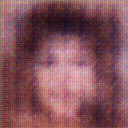
\includegraphics[width=150px]{500_fake_images/samples_5_211.png}%
\caption{A Close Up Of A Person Holding A Tooth Brush}%
\end{figure}

%
\end{document}